%%%%%%%%%%%%%%%%%%%%%%%%%%%%%%%%%%%%%%%%%
% Otto-Friedrich-University of Bamberg
% Chair of Explainable Machine Learning (xAI)
% Deep Learning Assignments
% LaTeX Template
% Version 1.0
%
% Author:
% Sebastian Dörrich
%%%%%%%%%%%%%%%%%%%%%%%%%%%%%%%%%%%%%%%%%

\renewcommand\thesection{\arabic{section}}
\renewcommand\thesubsection{\thesection.\arabic{subsection}}

%----------------------------------------------------------------------------------------
% Directed Acyclic Graph
%----------------------------------------------------------------------------------------
\section{Directed Acyclic Graph [10 points]}
One important property for a feed-forward network, as discussed in the lectures, is that it must be a directed acyclic graph (DAG). A \textit{DAG is a directed graph that contains no directed cycles}. We will study some of its properties in this question.
\\\\
Let's define a graph $G=(V, E)$ in which $V$ is the set of all nodes as $\{v_1, v_2, ..., v_i, ... v_n\}$ and $E$ is the set of 
edges $E = \big\{e_{i,j} = (v_i, v_j) \mid v_i, v_j \in V \big\}$.
\\\\
A \textit{topological order of a directed graph} $G=(V, E)$ is an ordering of its nodes as $\{v_1, v_2, ..., v_i, ... v_n\}$ so that for every edge $(v_i, v_j)$ we have $i < j$.
\\\\
There are several lemmas that can be inferred from the definition of a DAG. One lemma is: if $G$ is a DAG, then $G$ has a node with no incoming edges.

\medskip

\subsection{G is a DAG then G has a Topological Ordering [2 points]}
Prove that if the graph $G$ is a DAG, then $G$ has a topological ordering.


\taskbreak

\subsection{G has a Topological Ordering then G is a DAG [2 points]}
Prove that if the graph $G$ has a topological order, then $G$ is a DAG.

\taskbreak

\subsection{Computational Graphs and Backpropagation [6 points]}
For the given expression:
\begin{equation}
    A = 2\cdot \left((a + b) \cdot (a - b)\right)
\end{equation}

\vspace{0.5cm}

We can introduce intermediate variables such that there is a single mathematical operation per assignment such as:
\begin{align}
    t_1 &= a + b & t_2 &= a - b & t_3 &= t_1 \cdot t_2 & A &= 2 \cdot t_3
\end{align}

\vspace{0.5cm}

We can then use that to draw the corresponding computation graph based on the introduced variables as shown in Figure \ref{fig:computation_graph}:
\begin{figure}[h!]
    \centering
    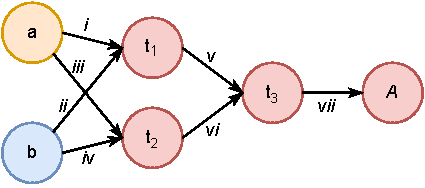
\includegraphics[scale=1.5]{./img/theory/ComputationGraph.pdf}
    \caption{Computation Graph based on the introduced intermediate variables.}
    \label{fig:computation_graph}
\end{figure}

\vspace{0.5cm}

Having the computation graph, we can write down the products of partial derivatives that are computed by a node during backpropagation for all of our nodes. Indicating to which node the results are sent to we can write:
\begin{equation}
    \begin{aligned}
        vii &\coloneqq \frac{\partial A}{\partial A} \frac{\partial A}{\partial t_3} & vi &\coloneqq \frac{\partial A}{\partial t_3} \frac{\partial t_3}{\partial t_2} & v &\coloneqq \frac{\partial A}{\partial t_3} \frac{\partial t_3}{\partial t_1} \\
        iv &\coloneqq \frac{\partial A}{\partial t_2} \frac{\partial t_2}{\partial b} &  iii &\coloneqq \frac{\partial A}{\partial t_2} \frac{\partial t_2}{\partial a} &  ii &\coloneqq \frac{\partial A}{\partial t_1} \frac{\partial t_1}{\partial b} \\
        i &\coloneqq \frac{\partial A}{\partial t_1} \frac{\partial t_1}{\partial a}
    \end{aligned}
\end{equation}

\vspace{0.5cm}

With this we can now write down the sum of partial derivative products that calculates the derivative of
the output node w.r.t. to this node for all of our nodes as:
\begin{equation}
    \begin{aligned}
        A&: \frac{\partial A}{\partial A} & t_3&: \frac{\partial A}{\partial t_3} & t_2&: \frac{\partial A}{\partial t_2} & t_1&: \frac{\partial A}{\partial t_1} \\\\
        \phantom{a}&\phantom{\frac{\partial A}{\partial t_2} \frac{\partial t_2}{\partial a} + \frac{\partial A}{\partial t_1} \frac{\partial t_1}{\partial a}} & b&: \frac{\partial A}{\partial t_2} \frac{\partial t_2}{\partial b} + \frac{\partial A}{\partial t_1} \frac{\partial t_1}{\partial b} & a&: \frac{\partial A}{\partial t_2} \frac{\partial t_2}{\partial a} + \frac{\partial A}{\partial t_1} \frac{\partial t_1}{\partial a}
    \end{aligned}
\end{equation}

\newpage

Now it is your turn. Given is the expressions:
\begin{equation}
    \begin{aligned}
        A &= \frac{{\rm e}^{a}}{\sqrt{b}} \log \left(a + b\right) \\
        % B &= \sqrt{a + b + c^2} + \log\left(a + b + c^2 \right) + \frac{a + b + c^2}{bc^2} \\
        % C &= \sum_{i=1}^{3} \left(w_0 + w_1 x_i - y_i \right)^2
    \end{aligned}
\end{equation}
\begin{itemize}
    \item[a)] Introduce intermediate variables ($t_1$, $t_2$, $t_3$, ...) such that there is a single mathematical operation per assignment. Reuse intermediate variables whenever possible.
    \subtaskbreak

    \item[b)] Draw the corresponding computation graph based on the variables you introduced in a).
    \subtaskbreak
    
    \item[c)] For each edge in your computation graph, write down the products of partial derivatives $\left(\text{e.g. } \frac{\partial \mathcal{L}}{\partial y} \frac{\partial y}{\partial x}\right)$ that are computed by this edge during backpropagation. For each such product indicate to which node the results are sent to (e.g. by writing down the products close to the corresponding graph edges).\\
    Note: you do not need to symbolically calculate or simplify the derivative for specific operations.
    \subtaskbreak
    
    \item[d)] At each node, write down the sum of partial derivative products that calculates the derivative of the output node w.r.t. to this node. Your expressions only need to contain the direct children for the node and again you do not need to symbolically calculate or simplify the derivatives.
\end{itemize}

